\chapter{Implementation}

This chapter focus on the implementation details of two add-ons:
\begin{enumerate}
\item a malicious add-on, which can infect the victim`s filesystem
\item a Transcriptase detection add-on, which can detect the metamorphic malware embedded in the web page.
\end{enumerate}

\section{Malicious add-on}

Generally browsers like Firefox, Chrome, and Opera do not allow access to the client filesystem using JavaScript. Even though creating a file is possible in IE using ActiveX objects, the client must enable ActiveX scripts on their system for the ActiveX object related code to execute properly [36]. 

Firefox add-ons are very powerful because of the high-level APIs that the SDK provides. The SDK has a file I/O module which provides access to the client`s filesystem.

A malicious add-on was created to demonstrate the way that a victim`s machine may get infected by a malicious add-on. The basic functionality of this add-on is it provides the statistic value i.e., the total JavaScript bytes in the page loaded by the user as shown in the Figure ~\ref{fig:maliciousaddon}.

\begin{figure}
    \centering    
    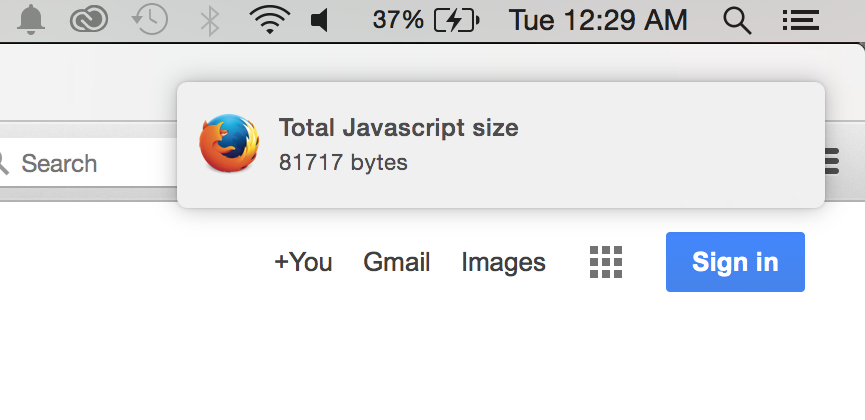
\includegraphics[width=8cm, height=3.9cm]{maliciousaddon.png}
    \caption[Main Functionality of the malicious add-on]{Main Functionality of the malicious add-on}
    \label{fig:maliciousaddon}
\end{figure}

The user expects this functionality and installs the malicious add-on, but this add-on also has hidden functionality. Whenever it finds that web page content has Transcriptase in it, it finds all the JavaScript files present in the filesystem and prepends them with Transcriptase code and thus it infects the victim`s filesystem. 

\begin{figure}
    \centering    
    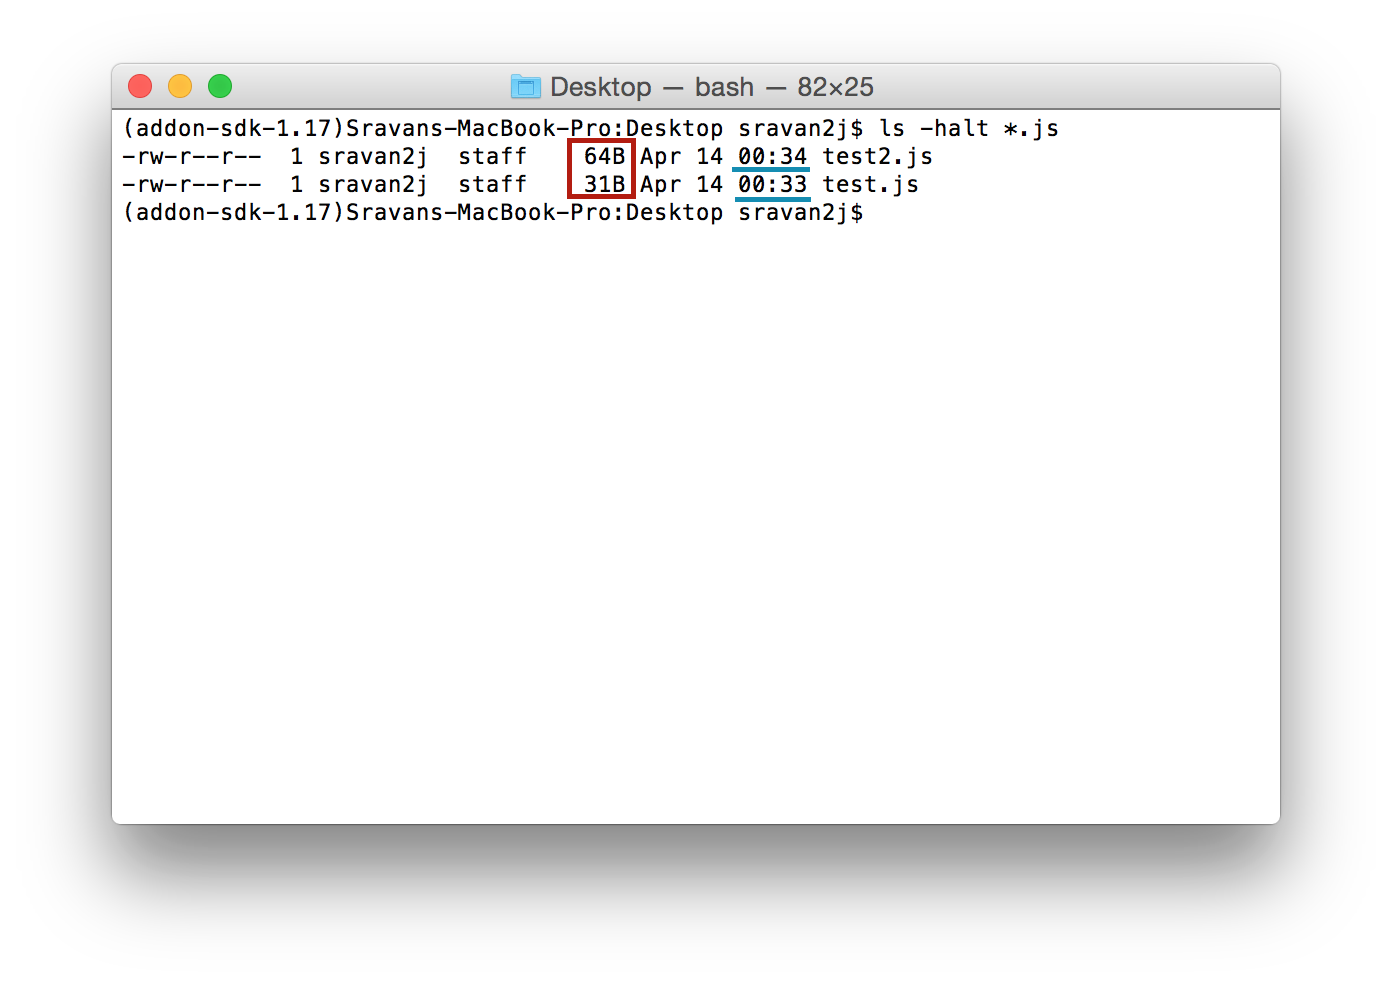
\includegraphics[width=17cm, height=11.95cm]{beforeinf.png}
    \caption[Size of sample JavaScript files before infection, ]{Size of sample JavaScript files before infection}
    \label{fig:beforeinf}
\end{figure}
\begin{figure}
    \centering    
    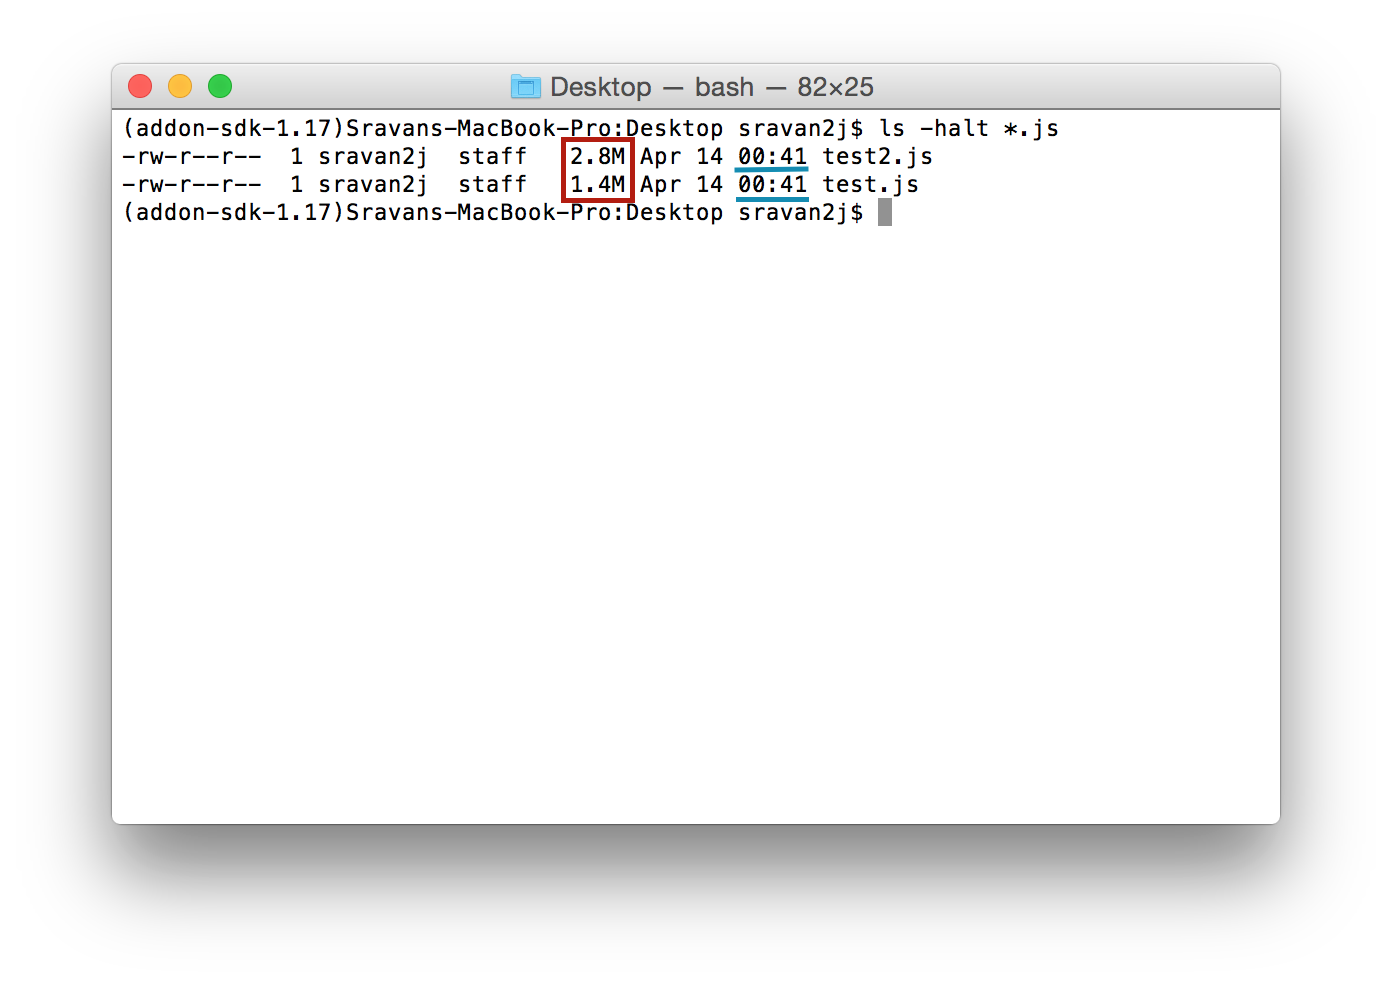
\includegraphics[width=17cm, height=11.95cm]{afterinf.png}
    \caption[JavaScript file sizes after infection]{JavaScript file sizes after infection}
    \label{fig:afterinf}
\end{figure}

Figure~\ref{fig:beforeinf} shows the size of our sample JavaScript files before infection and figure~\ref{fig:afterinf} shows the size of these files after infection. There is a huge difference in file sizes before and after infection. This infection will remain unknown to the user until the infected files are checked.

\section{Transcriptase detection add-on} 

\textbf{——— BELOW DATA IS JUNK DATA ——–}

	
\LaTeX\ can be viewed
as a compiled programming language, in contrast to that 
nightmare known as Microsoft Word,
which can be viewed as an interpreted language. So, to typeset a
document in \LaTeX, you create a text file that has the {\tt .tex} extension.
This file includes some special
commands, known as macros. Then
you compile your {\tt .tex} file by running  \LaTeX,
which produces your typeset document, as a pdf. 

In this paper, a few basics are discussed. There are plenty of good online resource
if you need help with more advanced topics.


\section{Opcode Graph Similarity} 

To typeset text, you type whatever you want. Multiple spaces are
ignored                           when typesetting, and
the end of a line is treated as another space.
Consequently, when you are typing, you can break lines anywhere, like here
or here,
since the lines are formatted automatically when you typeset the document.
You start a new paragraph by leaving a blank line.

See how easy it is to start a new paragraph? A blank line does the trick.


